\documentclass[12pt]{beamer}
\usetheme{Warsaw}
\usepackage[utf8]{inputenc}
\usepackage{amsmath}
\usepackage{amsfonts}
\usepackage{amssymb}
\usepackage{graphicx}
\usepackage[font=Times,timeinterval=1,timeduration=2.0,timedeath=0,fillcolorwarningsecond=white!60!yellow,timewarningfirst=50,timewarningsecond=80,resetatpages=2]{tdclock}
\usepackage{tabularx}
\usepackage{array}
\usepackage{multicol}
\usepackage{longtable}
\usepackage{xcolor}
\usepackage{textcomp, gensymb}
\usepackage{pgfplots}
\usepackage[makeroom]{cancel}

\graphicspath{ {./references/} }
\pgfplotsset{
	soldot/.style={color=black,only marks,mark=*},
	holdot/.style={color=black,fill=white,only marks,mark=*},
	compat=1.12
}
\newcolumntype{Y}{>{\centering\arraybackslash}X}
\makeatletter
\def\@listii{\leftmargin\leftmarginii
			  \topsep    2ex
			  \parsep    0\p@   \@plus\p@
			  \itemsep   \parsep}
\makeatother
\newcommand\at[2]{\left.#1\right|_{#2}}

\begin{document}
\begin{frame}
	\frametitle{Bellwork 12/14}
	\initclock

	Compute the area under $f(x)=\frac{1}{x}+1$ on $[1, 7]$ using a right Riemann sum with $\Delta x=2$.
	\vfill
	\begin{center}
		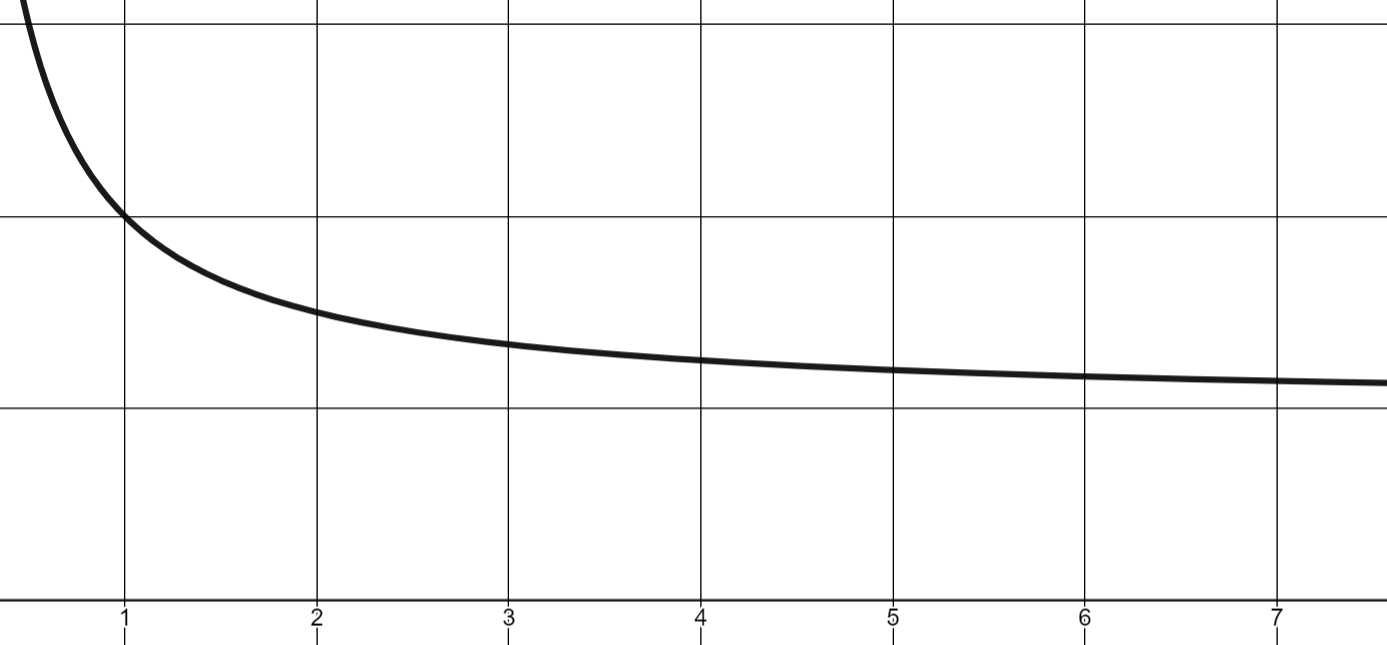
\includegraphics[scale=0.35]{bellwork_graph.png}
	\end{center}
	\vfill

	\small
	\crono
	\resetcrono{\beamerbutton{reset}}
\end{frame}
\begin{frame}
	\frametitle{Exercise 1}

	\vfill
	\Large
	\begin{table}[]
		\begin{tabular}{|l|r|r|r|r|}
			\hline
			x    & \quad-1 & \quad2 & \quad3 & \quad6 \\ \hline
			f(x) & \quad4  & \quad8 & \quad9 & \quad7 \\ \hline
		\end{tabular}
	\end{table}\par
	\vfill
	\vfill
	\large
	Using 3 sub-intervals, estimate $\int_{-1}^{6}f(x)dx$ with a:
	\vfill
	\begin{enumerate}\itemsep2ex
		\item Left Riemann sum
		\item Right Riemann sum
		\item Trapezoid sum
	\end{enumerate}
\end{frame}
\end{document}